% Shared preamble: packages, margins, and the \resume* macros.
%-------------------------
% Resume in Latex
% Author : Jake Gutierrez
% Based off of: https://github.com/sb2nov/resume
% License : MIT
%------------------------

\documentclass[letterpaper,11pt]{article}
\usepackage[T1]{fontenc}
\usepackage{latexsym}
\usepackage[empty]{fullpage}
\usepackage{titlesec}
\usepackage{marvosym}
\usepackage[usenames,dvipsnames]{color}
\usepackage{verbatim}
\usepackage{enumitem}
\usepackage[hidelinks]{hyperref}
\usepackage{fancyhdr}
\usepackage[english]{babel}
\usepackage{tabularx}
\usepackage[pro]{fontawesome5}
\usepackage{graphicx}
\usepackage{tikz}
\usepackage{hyperref}
\usepackage{bold-extra}
\usepackage{multirow}
\usepackage{xparse}

\hypersetup{
    colorlinks=true,
    linkcolor=blue,
    filecolor=magenta,      
    urlcolor=blue,
    pdftitle={CV - Delyan Boychev},
    pdfpagemode=FullScreen,
    }
\input{glyphtounicode}


%----------FONT OPTIONS----------
% sans-serif
% \usepackage[sfdefault]{FiraSans}
% \usepackage[sfdefault]{roboto}
% \usepackage[sfdefault]{noto-sans}
% \usepackage[default]{sourcesanspro}

% serif
% \usepackage{CormorantGaramond}
% \usepackage{charter}


\pagestyle{fancy}
\fancyhf{} % clear all header and footer fields
\fancyfoot{}
\renewcommand{\headrulewidth}{0pt}
\renewcommand{\footrulewidth}{0pt}

% Adjust margins
\addtolength{\oddsidemargin}{-0.5in}
\addtolength{\evensidemargin}{-0.5in}
\addtolength{\textwidth}{1in}
\addtolength{\topmargin}{-.5in}
\addtolength{\textheight}{1.0in}

\urlstyle{same}

\raggedbottom
\raggedright
\setlength{\tabcolsep}{0in}
\setlength{\footskip}{5pt}

% Sections formatting
\titleformat{\section}{
  \vspace{-4pt}\scshape\raggedright\large
}{}{0em}{}[\color{black}\titlerule \vspace{-5pt}]

% Ensure that generate pdf is machine readable/ATS parsable
\pdfgentounicode=1

%-------------------------
% Custom commands
\newcommand{\resumeItem}[1]{
  \item\small{#1}\vspace{-2pt}
}

% Width of the entry headings: the full text block minus the list indent, so the
% right-hand column (locations, dates) ends flush with the section rules.
\newcommand{\headingwidth}{\dimexpr\textwidth-0.15in\relax}

\newcommand{\resumeSubheading}[4]{
  \vspace{-2pt}\item
    \begin{tabular*}{\headingwidth}[t]{l@{\extracolsep{\fill}}r}
      \textbf{#1} & #2 \\
      \textit{\small#3} & \textit{\small #4} \\
    \end{tabular*}\vspace{-7pt}
}

\newcommand{\resumeSubSubheading}[2]{
    \item
    \begin{tabular*}{\headingwidth}{l@{\extracolsep{\fill}}r}
      \textit{\small#1} & \textit{\small #2} \\
    \end{tabular*}\vspace{-7pt}
}

\newcommand{\resumeProjectHeading}[3]{
    \item
    \begin{tabular*}{\headingwidth}{l@{\extracolsep{\fill}}r}
      \small #1 & #2 \\
      \ifx\relax#3\relax \else \textit{#3} & \\ \fi
    \end{tabular*}\vspace{-7pt}
}

\newcommand{\resumeSubItem}[1]{\resumeItem{#1}\vspace{-4pt}}

% Uniform link bullets: \cvlink{Label}{url}{shown text}, joined with \linksep
\newcommand{\cvlink}[3]{\textbf{#1:} \href{#2}{#3}}
\newcommand{\linksep}{\hspace{1.5mm}\textbar\hspace{1.5mm}}

\renewcommand\labelitemii{$\vcenter{\hbox{\tiny$\bullet$}}$}

\newcommand{\resumeSubHeadingListStart}{\begin{itemize}[leftmargin=0.15in, label={}]}
\newcommand{\resumeSubHeadingListEnd}{\end{itemize}}
\newcommand{\resumeItemListStart}{\begin{itemize}}
% Compact variant for the standalone bullet sections (interests, honors, skills)
\newcommand{\resumeFlatListStart}{\begin{itemize}[itemsep=1pt, parsep=0pt, topsep=2pt, partopsep=0pt]}
\newcommand{\resumeFlatListEnd}{\end{itemize}\vspace{-5pt}}
\newcommand{\resumeItemListEnd}{\end{itemize}\vspace{-5pt}}

%-------------------------------------------


%%%%%%  RESUME STARTS HERE  %%%%%%%%%%%%%%%%%%%%%%%%%%%%


\begin{document}

%----------HEADING----------
% \begin{tabular*}{\textwidth}{l@{\extracolsep{\fill}}r}
%   \textbf{\href{http://sourabhbajaj.com/}{\Large Sourabh Bajaj}} & Email : \href{mailto:sourabh@sourabhbajaj.com}{sourabh@sourabhbajaj.com}\\
%   \href{http://sourabhbajaj.com/}{http://www.sourabhbajaj.com} & Mobile : +1-123-456-7890 \\
% \end{tabular*}

% Shared header: photo, name, and contact links.
\begin{minipage}{0.15\textwidth}%
\begin{tikzpicture}
\clip[rounded corners=6pt] (-1.4,-1.4) rectangle (1.4,1.4);
\node[anchor=center] at (0,-0.2) {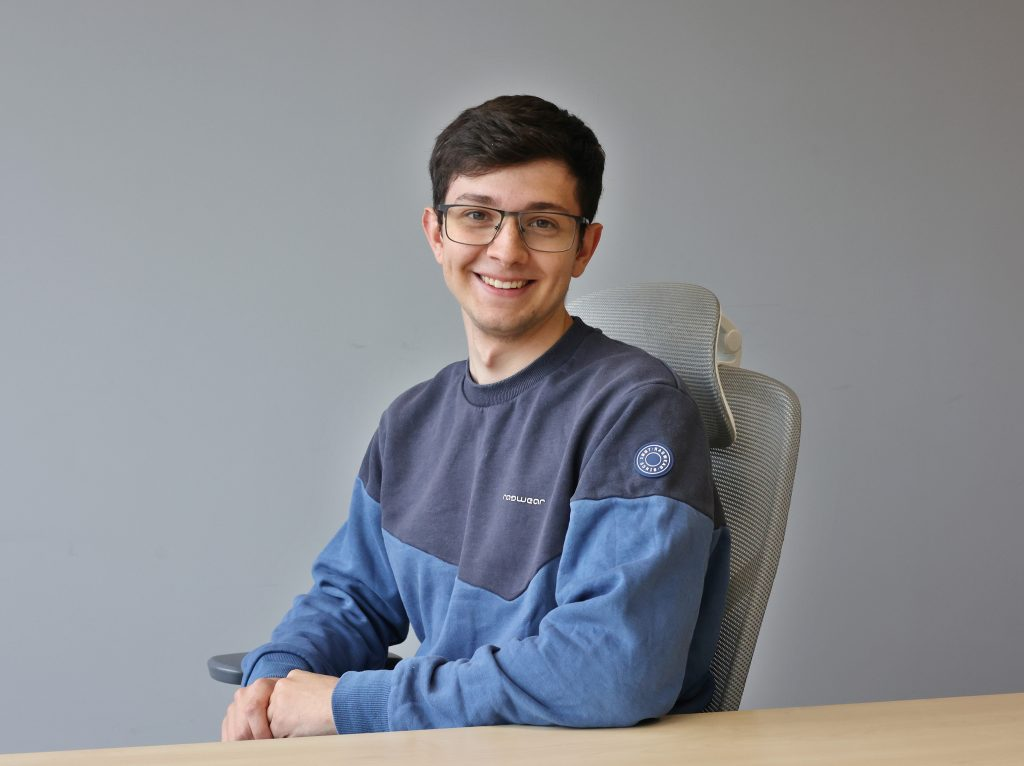
\includegraphics[width=4.5cm]{photo.jpg}};
%adjust this coordinate to move image
\end{tikzpicture}
\end{minipage}\hspace{10pt}
\begin{minipage}{0.8\textwidth}%
 \textbf{\Huge \scshape Delyan Boychev} \\ \vspace{1pt}
    \small \faAt \hspace{0.5mm} \href{mailto:delyan.boychev@insait.ai}{delyan.boychev@insait.ai} $|$ \faLinkedin \hspace{0.5mm}
    \href{https://www.linkedin.com/in/d-boychev/}{d-boychev} $|$ \faGithub \hspace{0.5mm}
    \href{https://github.com/delyan-boychev/}{delyan-boychev} $|$ \faBookOpen\hspace{0.5mm}\href{https://scholar.google.com/citations?user=_uql_SsAAAAJ&hl=en}{Scholar} $|$ \faGlobe \hspace{0.5mm}
    \href{https://dboychev.com}{dboychev.com}
    \vspace{1mm}\\
    Sofia, Bulgaria
\end{minipage}


\section{\texorpdfstring{\faUser}{} About me}

% Default summary. A tailored variant (e.g. main-incidentio.tex) defines \aboutme
% before % Shared preamble: packages, margins, and the \resume* macros.
%-------------------------
% Resume in Latex
% Author : Jake Gutierrez
% Based off of: https://github.com/sb2nov/resume
% License : MIT
%------------------------

\documentclass[letterpaper,11pt]{article}
\usepackage[T1]{fontenc}
\usepackage{latexsym}
\usepackage[empty]{fullpage}
\usepackage{titlesec}
\usepackage{marvosym}
\usepackage[usenames,dvipsnames]{color}
\usepackage{verbatim}
\usepackage{enumitem}
\usepackage[hidelinks]{hyperref}
\usepackage{fancyhdr}
\usepackage[english]{babel}
\usepackage{tabularx}
\usepackage[pro]{fontawesome5}
\usepackage{graphicx}
\usepackage{tikz}
\usepackage{hyperref}
\usepackage{bold-extra}
\usepackage{multirow}
\usepackage{xparse}

\hypersetup{
    colorlinks=true,
    linkcolor=blue,
    filecolor=magenta,      
    urlcolor=blue,
    pdftitle={CV - Delyan Boychev},
    pdfpagemode=FullScreen,
    }
\input{glyphtounicode}


%----------FONT OPTIONS----------
% sans-serif
% \usepackage[sfdefault]{FiraSans}
% \usepackage[sfdefault]{roboto}
% \usepackage[sfdefault]{noto-sans}
% \usepackage[default]{sourcesanspro}

% serif
% \usepackage{CormorantGaramond}
% \usepackage{charter}


\pagestyle{fancy}
\fancyhf{} % clear all header and footer fields
\fancyfoot{}
\renewcommand{\headrulewidth}{0pt}
\renewcommand{\footrulewidth}{0pt}

% Adjust margins
\addtolength{\oddsidemargin}{-0.5in}
\addtolength{\evensidemargin}{-0.5in}
\addtolength{\textwidth}{1in}
\addtolength{\topmargin}{-.5in}
\addtolength{\textheight}{1.0in}

\urlstyle{same}

\raggedbottom
\raggedright
\setlength{\tabcolsep}{0in}
\setlength{\footskip}{5pt}

% Sections formatting
\titleformat{\section}{
  \vspace{-4pt}\scshape\raggedright\large
}{}{0em}{}[\color{black}\titlerule \vspace{-5pt}]

% Ensure that generate pdf is machine readable/ATS parsable
\pdfgentounicode=1

%-------------------------
% Custom commands
\newcommand{\resumeItem}[1]{
  \item\small{#1}\vspace{-2pt}
}

% Width of the entry headings: the full text block minus the list indent, so the
% right-hand column (locations, dates) ends flush with the section rules.
\newcommand{\headingwidth}{\dimexpr\textwidth-0.15in\relax}

\newcommand{\resumeSubheading}[4]{
  \vspace{-2pt}\item
    \begin{tabular*}{\headingwidth}[t]{l@{\extracolsep{\fill}}r}
      \textbf{#1} & #2 \\
      \textit{\small#3} & \textit{\small #4} \\
    \end{tabular*}\vspace{-7pt}
}

\newcommand{\resumeSubSubheading}[2]{
    \item
    \begin{tabular*}{\headingwidth}{l@{\extracolsep{\fill}}r}
      \textit{\small#1} & \textit{\small #2} \\
    \end{tabular*}\vspace{-7pt}
}

\newcommand{\resumeProjectHeading}[3]{
    \item
    \begin{tabular*}{\headingwidth}{l@{\extracolsep{\fill}}r}
      \small #1 & #2 \\
      \ifx\relax#3\relax \else \textit{#3} & \\ \fi
    \end{tabular*}\vspace{-7pt}
}

\newcommand{\resumeSubItem}[1]{\resumeItem{#1}\vspace{-4pt}}

% Uniform link bullets: \cvlink{Label}{url}{shown text}, joined with \linksep
\newcommand{\cvlink}[3]{\textbf{#1:} \href{#2}{#3}}
\newcommand{\linksep}{\hspace{1.5mm}\textbar\hspace{1.5mm}}

\renewcommand\labelitemii{$\vcenter{\hbox{\tiny$\bullet$}}$}

\newcommand{\resumeSubHeadingListStart}{\begin{itemize}[leftmargin=0.15in, label={}]}
\newcommand{\resumeSubHeadingListEnd}{\end{itemize}}
\newcommand{\resumeItemListStart}{\begin{itemize}}
% Compact variant for the standalone bullet sections (interests, honors, skills)
\newcommand{\resumeFlatListStart}{\begin{itemize}[itemsep=1pt, parsep=0pt, topsep=2pt, partopsep=0pt]}
\newcommand{\resumeFlatListEnd}{\end{itemize}\vspace{-5pt}}
\newcommand{\resumeItemListEnd}{\end{itemize}\vspace{-5pt}}

%-------------------------------------------


%%%%%%  RESUME STARTS HERE  %%%%%%%%%%%%%%%%%%%%%%%%%%%%


\begin{document}

%----------HEADING----------
% \begin{tabular*}{\textwidth}{l@{\extracolsep{\fill}}r}
%   \textbf{\href{http://sourabhbajaj.com/}{\Large Sourabh Bajaj}} & Email : \href{mailto:sourabh@sourabhbajaj.com}{sourabh@sourabhbajaj.com}\\
%   \href{http://sourabhbajaj.com/}{http://www.sourabhbajaj.com} & Mobile : +1-123-456-7890 \\
% \end{tabular*}

% Shared header: photo, name, and contact links.
\begin{minipage}{0.15\textwidth}%
\begin{tikzpicture}
\clip[rounded corners=6pt] (-1.4,-1.4) rectangle (1.4,1.4);
\node[anchor=center] at (0,-0.2) {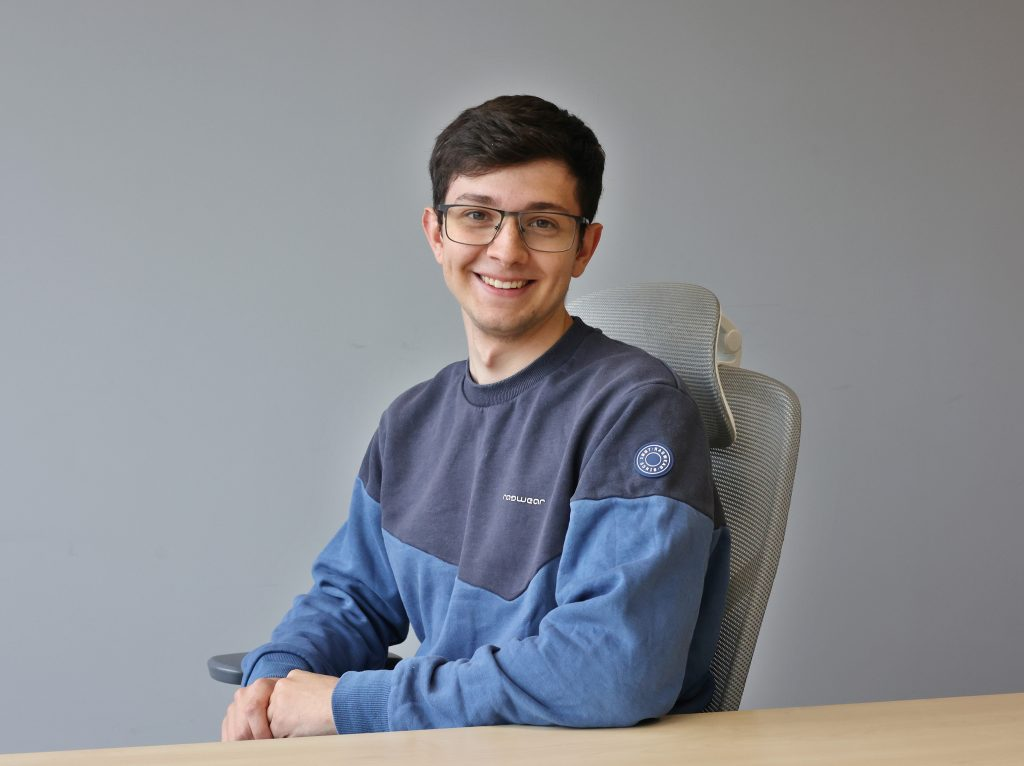
\includegraphics[width=4.5cm]{photo.jpg}};
%adjust this coordinate to move image
\end{tikzpicture}
\end{minipage}\hspace{10pt}
\begin{minipage}{0.8\textwidth}%
 \textbf{\Huge \scshape Delyan Boychev} \\ \vspace{1pt}
    \small \faAt \hspace{0.5mm} \href{mailto:delyan.boychev@insait.ai}{delyan.boychev@insait.ai} $|$ \faLinkedin \hspace{0.5mm}
    \href{https://www.linkedin.com/in/d-boychev/}{d-boychev} $|$ \faGithub \hspace{0.5mm}
    \href{https://github.com/delyan-boychev/}{delyan-boychev} $|$ \faBookOpen\hspace{0.5mm}\href{https://scholar.google.com/citations?user=_uql_SsAAAAJ&hl=en}{Scholar} $|$ \faGlobe \hspace{0.5mm}
    \href{https://dboychev.com}{dboychev.com}
    \vspace{1mm}\\
    Sofia, Bulgaria
\end{minipage}


\section{\texorpdfstring{\faUser}{} About me}

% Default summary. A tailored variant (e.g. main-incidentio.tex) defines \aboutme
% before % Shared preamble: packages, margins, and the \resume* macros.
%-------------------------
% Resume in Latex
% Author : Jake Gutierrez
% Based off of: https://github.com/sb2nov/resume
% License : MIT
%------------------------

\documentclass[letterpaper,11pt]{article}
\usepackage[T1]{fontenc}
\usepackage{latexsym}
\usepackage[empty]{fullpage}
\usepackage{titlesec}
\usepackage{marvosym}
\usepackage[usenames,dvipsnames]{color}
\usepackage{verbatim}
\usepackage{enumitem}
\usepackage[hidelinks]{hyperref}
\usepackage{fancyhdr}
\usepackage[english]{babel}
\usepackage{tabularx}
\usepackage[pro]{fontawesome5}
\usepackage{graphicx}
\usepackage{tikz}
\usepackage{hyperref}
\usepackage{bold-extra}
\usepackage{multirow}
\usepackage{xparse}

\hypersetup{
    colorlinks=true,
    linkcolor=blue,
    filecolor=magenta,      
    urlcolor=blue,
    pdftitle={CV - Delyan Boychev},
    pdfpagemode=FullScreen,
    }
\input{glyphtounicode}


%----------FONT OPTIONS----------
% sans-serif
% \usepackage[sfdefault]{FiraSans}
% \usepackage[sfdefault]{roboto}
% \usepackage[sfdefault]{noto-sans}
% \usepackage[default]{sourcesanspro}

% serif
% \usepackage{CormorantGaramond}
% \usepackage{charter}


\pagestyle{fancy}
\fancyhf{} % clear all header and footer fields
\fancyfoot{}
\renewcommand{\headrulewidth}{0pt}
\renewcommand{\footrulewidth}{0pt}

% Adjust margins
\addtolength{\oddsidemargin}{-0.5in}
\addtolength{\evensidemargin}{-0.5in}
\addtolength{\textwidth}{1in}
\addtolength{\topmargin}{-.5in}
\addtolength{\textheight}{1.0in}

\urlstyle{same}

\raggedbottom
\raggedright
\setlength{\tabcolsep}{0in}
\setlength{\footskip}{5pt}

% Sections formatting
\titleformat{\section}{
  \vspace{-4pt}\scshape\raggedright\large
}{}{0em}{}[\color{black}\titlerule \vspace{-5pt}]

% Ensure that generate pdf is machine readable/ATS parsable
\pdfgentounicode=1

%-------------------------
% Custom commands
\newcommand{\resumeItem}[1]{
  \item\small{#1}\vspace{-2pt}
}

% Width of the entry headings: the full text block minus the list indent, so the
% right-hand column (locations, dates) ends flush with the section rules.
\newcommand{\headingwidth}{\dimexpr\textwidth-0.15in\relax}

\newcommand{\resumeSubheading}[4]{
  \vspace{-2pt}\item
    \begin{tabular*}{\headingwidth}[t]{l@{\extracolsep{\fill}}r}
      \textbf{#1} & #2 \\
      \textit{\small#3} & \textit{\small #4} \\
    \end{tabular*}\vspace{-7pt}
}

\newcommand{\resumeSubSubheading}[2]{
    \item
    \begin{tabular*}{\headingwidth}{l@{\extracolsep{\fill}}r}
      \textit{\small#1} & \textit{\small #2} \\
    \end{tabular*}\vspace{-7pt}
}

\newcommand{\resumeProjectHeading}[3]{
    \item
    \begin{tabular*}{\headingwidth}{l@{\extracolsep{\fill}}r}
      \small #1 & #2 \\
      \ifx\relax#3\relax \else \textit{#3} & \\ \fi
    \end{tabular*}\vspace{-7pt}
}

\newcommand{\resumeSubItem}[1]{\resumeItem{#1}\vspace{-4pt}}

% Uniform link bullets: \cvlink{Label}{url}{shown text}, joined with \linksep
\newcommand{\cvlink}[3]{\textbf{#1:} \href{#2}{#3}}
\newcommand{\linksep}{\hspace{1.5mm}\textbar\hspace{1.5mm}}

\renewcommand\labelitemii{$\vcenter{\hbox{\tiny$\bullet$}}$}

\newcommand{\resumeSubHeadingListStart}{\begin{itemize}[leftmargin=0.15in, label={}]}
\newcommand{\resumeSubHeadingListEnd}{\end{itemize}}
\newcommand{\resumeItemListStart}{\begin{itemize}}
% Compact variant for the standalone bullet sections (interests, honors, skills)
\newcommand{\resumeFlatListStart}{\begin{itemize}[itemsep=1pt, parsep=0pt, topsep=2pt, partopsep=0pt]}
\newcommand{\resumeFlatListEnd}{\end{itemize}\vspace{-5pt}}
\newcommand{\resumeItemListEnd}{\end{itemize}\vspace{-5pt}}

%-------------------------------------------


%%%%%%  RESUME STARTS HERE  %%%%%%%%%%%%%%%%%%%%%%%%%%%%


\begin{document}

%----------HEADING----------
% \begin{tabular*}{\textwidth}{l@{\extracolsep{\fill}}r}
%   \textbf{\href{http://sourabhbajaj.com/}{\Large Sourabh Bajaj}} & Email : \href{mailto:sourabh@sourabhbajaj.com}{sourabh@sourabhbajaj.com}\\
%   \href{http://sourabhbajaj.com/}{http://www.sourabhbajaj.com} & Mobile : +1-123-456-7890 \\
% \end{tabular*}

% Shared header: photo, name, and contact links.
\begin{minipage}{0.15\textwidth}%
\begin{tikzpicture}
\clip[rounded corners=6pt] (-1.4,-1.4) rectangle (1.4,1.4);
\node[anchor=center] at (0,-0.2) {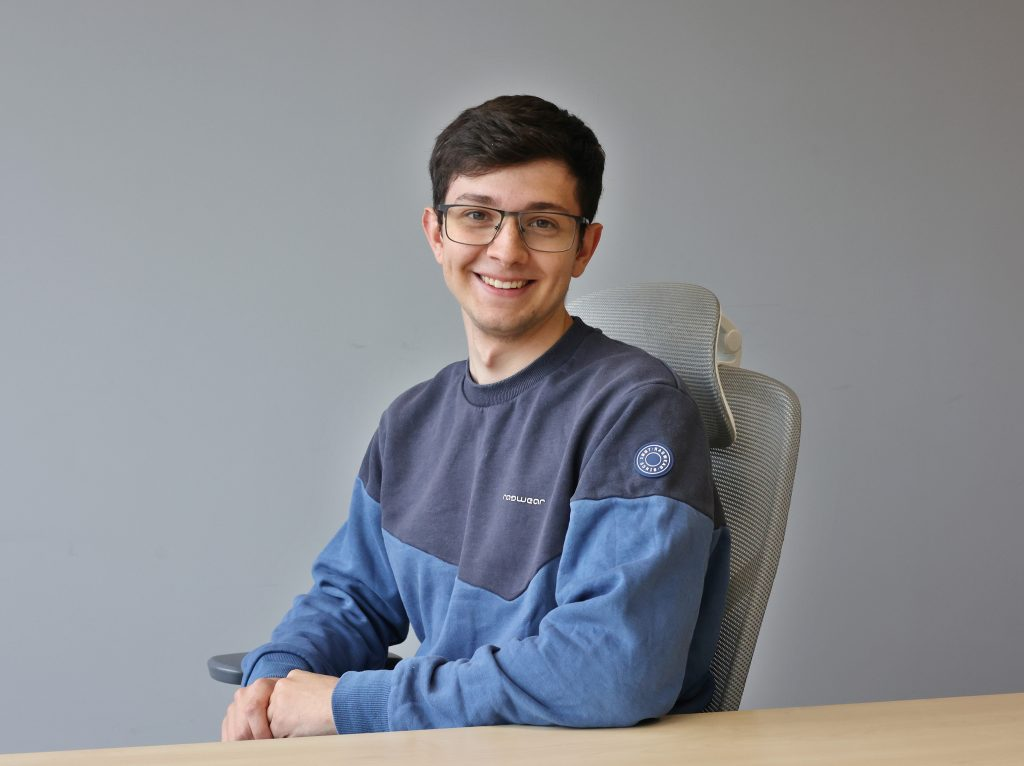
\includegraphics[width=4.5cm]{photo.jpg}};
%adjust this coordinate to move image
\end{tikzpicture}
\end{minipage}\hspace{10pt}
\begin{minipage}{0.8\textwidth}%
 \textbf{\Huge \scshape Delyan Boychev} \\ \vspace{1pt}
    \small \faAt \hspace{0.5mm} \href{mailto:delyan.boychev@insait.ai}{delyan.boychev@insait.ai} $|$ \faLinkedin \hspace{0.5mm}
    \href{https://www.linkedin.com/in/d-boychev/}{d-boychev} $|$ \faGithub \hspace{0.5mm}
    \href{https://github.com/delyan-boychev/}{delyan-boychev} $|$ \faBookOpen\hspace{0.5mm}\href{https://scholar.google.com/citations?user=_uql_SsAAAAJ&hl=en}{Scholar} $|$ \faGlobe \hspace{0.5mm}
    \href{https://dboychev.com}{dboychev.com}
    \vspace{1mm}\\
    Sofia, Bulgaria
\end{minipage}


\section{\texorpdfstring{\faUser}{} About me}

% Default summary. A tailored variant (e.g. main-incidentio.tex) defines \aboutme
% before % Shared preamble: packages, margins, and the \resume* macros.
\input{preamble.tex}

%%%%%%  RESUME STARTS HERE  %%%%%%%%%%%%%%%%%%%%%%%%%%%%


\begin{document}

%----------HEADING----------
% \begin{tabular*}{\textwidth}{l@{\extracolsep{\fill}}r}
%   \textbf{\href{http://sourabhbajaj.com/}{\Large Sourabh Bajaj}} & Email : \href{mailto:sourabh@sourabhbajaj.com}{sourabh@sourabhbajaj.com}\\
%   \href{http://sourabhbajaj.com/}{http://www.sourabhbajaj.com} & Mobile : +1-123-456-7890 \\
% \end{tabular*}

% Shared header: photo, name, and contact links.
\input{header.tex}

\section{\texorpdfstring{\faUser}{} About me}

% Default summary. A tailored variant (e.g. main-incidentio.tex) defines \aboutme
% before \input{main.tex} to swap this paragraph without duplicating the CV.
\providecommand{\aboutme}{Informatics undergraduate and INSAIT research scholar working on vision-language models, remote sensing, 3D scene understanding, and efficient transformer inference. IOAI lecturer; previously a Quant ML intern at Man Group and an NLP research intern at Graphwise. Research spans domain adaptation, synthetic-image detection, adversarial robustness, and interpretability.}
\aboutme

\vspace{-3mm}
%-----------EDUCATION-----------
\section{\texorpdfstring{\faGraduationCap}{} Education}
  \resumeSubHeadingListStart
  \resumeSubheading
      {\parbox[t]{0.72\textwidth}{\href{https://insait.ai/delyan-boychev/}{INSAIT Scholar} (\href{https://explorer.insait.ai/}{highly selective 4-year program}) \\ Faculty of Mathematics and Informatics, Sofia University}}{Sofia, Bulgaria}
      {\texorpdfstring{Bachelor of Informatics}{}}{Sept.\ 2024 -- Expected 2028}
  \resumeSubHeadingListEnd
\vspace{-3mm}
\section{\texorpdfstring{\faBriefcase}{} Experience}
    \resumeSubHeadingListStart
    \resumeProjectHeading{\textbf{NLP Research Intern \textbar \space Graphwise}}{July 2026 -- Sept.\ 2026}{}
    \resumeItemListStart
    \resumeItem{Built NLP pipelines for table entity reconciliation, knowledge-base linking, and structured extraction from unstructured text.}
    \resumeItem{Optimized language-model pipelines for deployment, improving inference cost and latency.}
    \resumeItemListEnd
    \resumeProjectHeading{\textbf{IOAI Lecturer \textbar \space Bulgarian IOAI Team}}{June 2025 -- Present}{}
    \resumeItemListStart
    \resumeItem{Lecturing and mentoring students preparing for the International Olympiad in Artificial Intelligence (IOAI).}
    \resumeItemListEnd
    \resumeProjectHeading{\textbf{Undergrad Research Scholar \textbar \space INSAIT}}{Oct.\ 2024 -- Present}{}
    \resumeItemListStart
    \resumeItem{Researching vision-language models for remote sensing and 3D scene understanding under the advisory of Dr. Danda Paudel.}
    \resumeItemListEnd
    \resumeProjectHeading{\textbf{Quant ML Intern \textbar \space {Man Group}}}{July 2025 -- Sept.\ 2025}{}
    \resumeItemListStart
    \resumeItem{Conducted Quant ML research, focusing on developing and evaluating machine-learning models for systematic trading and signal forecasting.}
    \resumeItemListEnd
    \resumeSubHeadingListEnd
\vspace{-3mm}
\section{\texorpdfstring{\faBook}{} Publications}
    \resumeSubHeadingListStart
      \resumeProjectHeading{\textbf{OSMDA: OpenStreetMap-based Domain Adaptation for Remote Sensing VLMs} $|$ \textit{arXiv Preprint, 2026}}{}{}
      \resumeItemListStart
        \resumeItem{Stefan Maria Ailuro, Mario Markov, Mohammad Mahdi, \textbf{Delyan Boychev}, Luc Van Gool, Danda Pani Paudel}
        \resumeItem{Self-contained domain adaptation using OpenStreetMap supervision without manual labels or a stronger external teacher; under review.}
        \resumeItem{\cvlink{Paper}{https://arxiv.org/abs/2603.11804}{arxiv.org/abs/2603.11804}}
      \resumeItemListEnd
      \resumeProjectHeading{\textbf{ImagiNet: A Multi-Content Benchmark for Synthetic Image Detection} $|$ \textit{AAAI 2025 Workshop Paper}}{}{}
      \resumeItemListStart
        \resumeItem{\textbf{Delyan Boychev}, Radostin Cholakov --- AAAI 2025 Workshop on Datasets and Evaluators of AI Safety}
        \resumeItem{A balanced 200K-image benchmark spanning four content types and multiple open and proprietary generators, with strong contrastive-learning baselines.}
        \resumeItem{\cvlink{Paper}{https://arxiv.org/abs/2407.20020}{arxiv.org/abs/2407.20020}}
      \resumeItemListEnd
      \resumeProjectHeading{\textbf{Interpretable Computer Vision Models through Adversarial Training} $|$ \textit{arXiv Preprint, 2023}}{}{}
      \resumeItemListStart
        \resumeItem{Single-author empirical study of how adversarial training changes learned representations and model interpretability.}
        \resumeItem{\cvlink{Paper}{https://arxiv.org/abs/2307.02500}{arxiv.org/abs/2307.02500}}
      \resumeItemListEnd
    \resumeSubHeadingListEnd
\vspace{-3mm}
\section{\texorpdfstring{\faFolderOpen}{} Projects}
    \resumeSubHeadingListStart
      \resumeProjectHeading{\textbf{DisentangledFlash} $|$ \textit{Triton Attention Kernel}}{Aug.\ 2026 -- Present}{}
      \resumeItemListStart
        \resumeItem{Fuses DeBERTa-v2/v3 attention into a streaming Triton kernel without materializing the full attention matrix.}
        \resumeItem{On H200 benchmarks: up to 2.33$\times$ faster and up to 91\% lower peak memory than Hugging Face Transformers eager.}
        \resumeItem{\cvlink{Code}{https://github.com/delyan-boychev/disentangled-flash}{github.com/delyan-boychev/disentangled-flash}\linksep\cvlink{PyPI}{https://pypi.org/project/disentangled-flash/}{pypi.org/project/disentangled-flash}}
      \resumeItemListEnd
      \resumeProjectHeading{\textbf{LavBench} $|$ \textit{ML Competition Platform}}{June 2026 -- Present}{}
      \resumeItemListStart
        \resumeItem{A secure, bilingual platform for machine-learning competitions, built for Bulgarian AI Olympiad selection and national contests.}
        \resumeItem{Runs notebook and Python submissions in hardened Docker sandboxes; provides live leaderboards, double-blind jury review, custom evaluators, and distributed workers.}
        \resumeItem{\cvlink{Code}{https://github.com/delyan-boychev/lavbench}{github.com/delyan-boychev/lavbench}\linksep\cvlink{Docs}{https://lavbench.readthedocs.io/latest/}{lavbench.readthedocs.io}}
      \resumeItemListEnd
      \resumeProjectHeading{\textbf{Generative Translation} $|$ \textit{Coursework in Information Search and Retrieval: Application of Deep Learning}}{Feb.\ 2026}{}
      \resumeItemListStart
        \resumeItem{Built a decoder-only PyTorch Transformer for Bulgarian-to-English translation with custom BPE, masked attention, KV caching, and beam search.}
        \resumeItem{Achieved 42.57 BLEU-4 with 12.26 test perplexity using beam search.}
        \resumeItem{\cvlink{Code}{https://github.com/delyan-boychev/gen-trans}{github.com/delyan-boychev/gen-trans}}
      \resumeItemListEnd
      \resumeProjectHeading{\textbf{Vision-Language Models for Satellite Imagery Understanding} $|$ \textit{Research at INSAIT}}{Dec.\ 2025 -- Present}{Advised by \href{https://insait.ai/dr-danda-paudel/}{Dr. Danda Paudel}}
  \resumeItemListStart
    \resumeItem{Adapting vision-language models to satellite imagery using scalable supervision derived from OpenStreetMap.}
  \resumeItemListEnd\resumeProjectHeading{\textbf{Spatial Modeling for Point-Cloud Understanding} $|$ \textit{Research at INSAIT}}{June 2025 -- Present}{Advised by \href{https://insait.ai/dr-danda-paudel/}{Dr. Danda Paudel}}
  \resumeItemListStart
    \resumeItem{Aligning 3D point-cloud and Gaussian representations for structured spatial reasoning and scene understanding.}
  \resumeItemListEnd
\resumeProjectHeading
  {\textbf{C++ Coursework} $|$ \emph{DSA and OOP Course Projects}}{2025}{}
  \resumeItemListStart
    \resumeItem{Built a dependency-aware expression solver with polymorphic tokenization and two-stack evaluation, and a modular digital audio workstation with timeline editing, effects, and audio I/O.}
    \resumeItem{\cvlink{Solver}{https://github.com/delyan-boychev/partial-solver}{partial-solver}\linksep\cvlink{Audio Workstation}{https://github.com/delyan-boychev/dig-audio-workstation}{dig-audio-workstation}}
  \resumeItemListEnd
  \resumeProjectHeading
  {\textbf{ImagiNet} $|$ \emph{Synthetic Image Dataset}}{2024}{}
  \resumeItemListStart
    \resumeItem{A 144 GB, 200K-image dataset for synthetic-image detection, balanced across photos, paintings, faces, and uncategorized imagery.}
    \resumeItem{Supports both real-versus-synthetic classification and generator identification across open and proprietary image generators.}
    \resumeItem{\cvlink{Dataset}{https://huggingface.co/datasets/delyanboychev/imaginet}{huggingface.co/datasets/delyanboychev/imaginet}}
  \resumeItemListEnd
  \resumeProjectHeading
  {\textbf{Gradient Cache Contrastive Learning} $|$ \emph{PyTorch Package}}{2023 -- 2024}{}
  \resumeItemListStart
    \resumeItem{A PyTorch implementation of gradient caching for scaling computer-vision contrastive learning beyond GPU memory limits.}
    \resumeItem{Reproduces large-batch gradients from smaller chunks; supports SimCLR, SupCon, SelfCon, mixed precision, and distributed training.}
    \resumeItem{\cvlink{Code}{https://github.com/delyan-boychev/grad-cache-con-learning}{github.com/delyan-boychev/grad-cache-con-learning}\linksep\cvlink{PyPI}{https://pypi.org/project/grad-cache-con-learning/}{pypi.org/project/grad-cache-con-learning}}
  \resumeItemListEnd
    \resumeSubHeadingListEnd
\vspace{-3mm}
\section{\texorpdfstring{\faAward}{} Honors}
\resumeFlatListStart
\resumeItem{Scholarship Recipient, EXPLORER Program, INSAIT (2024)}
\resumeItem{European Space Agency Award from EUCYS'24, Katowice, Poland}
\resumeItem{International Olympiad in Artificial Intelligence 2024, Team Bronze Medal}
\resumeItem{Regeneron ISEF'23 Finalist, Dallas, Texas}
\resumeItem{John Atanasoff Presidential Award in the category ``Debut breakthrough in computer technology'' (2023)}
\resumeFlatListEnd
\vspace{-1.5mm}
\section{\texorpdfstring{\faLaptopCode}{} Technical Skills}
\resumeFlatListStart
\resumeItem{\textbf{Languages:} Python, C++, TypeScript, JavaScript}
\resumeItem{\textbf{ML/Research:} PyTorch, Triton, vLLM, Hugging Face Transformers}
\resumeItem{\textbf{Data Science:} NumPy, pandas, scikit-learn}
\resumeItem{\textbf{Web \& Backend:} React, Vite, Tailwind CSS, Flask, Celery, PostgreSQL}
\resumeItem{\textbf{Tools:} Linux, Docker, Google Cloud, CI/CD, Git}
\resumeFlatListEnd
\vspace{-1.5mm}
\section{\texorpdfstring{\faLanguage}{} Languages}
\resumeFlatListStart
\resumeItem{Bulgarian --- Native}
\resumeItem{English --- IELTS Academic, 7.0/9.0}
\resumeFlatListEnd

%-------------------------------------------
\end{document}
 to swap this paragraph without duplicating the CV.
\providecommand{\aboutme}{Informatics undergraduate and INSAIT research scholar working on vision-language models, remote sensing, 3D scene understanding, and efficient transformer inference. IOAI lecturer; previously a Quant ML intern at Man Group and an NLP research intern at Graphwise. Research spans domain adaptation, synthetic-image detection, adversarial robustness, and interpretability.}
\aboutme

\vspace{-3mm}
%-----------EDUCATION-----------
\section{\texorpdfstring{\faGraduationCap}{} Education}
  \resumeSubHeadingListStart
  \resumeSubheading
      {\parbox[t]{0.72\textwidth}{\href{https://insait.ai/delyan-boychev/}{INSAIT Scholar} (\href{https://explorer.insait.ai/}{highly selective 4-year program}) \\ Faculty of Mathematics and Informatics, Sofia University}}{Sofia, Bulgaria}
      {\texorpdfstring{Bachelor of Informatics}{}}{Sept.\ 2024 -- Expected 2028}
  \resumeSubHeadingListEnd
\vspace{-3mm}
\section{\texorpdfstring{\faBriefcase}{} Experience}
    \resumeSubHeadingListStart
    \resumeProjectHeading{\textbf{NLP Research Intern \textbar \space Graphwise}}{July 2026 -- Sept.\ 2026}{}
    \resumeItemListStart
    \resumeItem{Built NLP pipelines for table entity reconciliation, knowledge-base linking, and structured extraction from unstructured text.}
    \resumeItem{Optimized language-model pipelines for deployment, improving inference cost and latency.}
    \resumeItemListEnd
    \resumeProjectHeading{\textbf{IOAI Lecturer \textbar \space Bulgarian IOAI Team}}{June 2025 -- Present}{}
    \resumeItemListStart
    \resumeItem{Lecturing and mentoring students preparing for the International Olympiad in Artificial Intelligence (IOAI).}
    \resumeItemListEnd
    \resumeProjectHeading{\textbf{Undergrad Research Scholar \textbar \space INSAIT}}{Oct.\ 2024 -- Present}{}
    \resumeItemListStart
    \resumeItem{Researching vision-language models for remote sensing and 3D scene understanding under the advisory of Dr. Danda Paudel.}
    \resumeItemListEnd
    \resumeProjectHeading{\textbf{Quant ML Intern \textbar \space {Man Group}}}{July 2025 -- Sept.\ 2025}{}
    \resumeItemListStart
    \resumeItem{Conducted Quant ML research, focusing on developing and evaluating machine-learning models for systematic trading and signal forecasting.}
    \resumeItemListEnd
    \resumeSubHeadingListEnd
\vspace{-3mm}
\section{\texorpdfstring{\faBook}{} Publications}
    \resumeSubHeadingListStart
      \resumeProjectHeading{\textbf{OSMDA: OpenStreetMap-based Domain Adaptation for Remote Sensing VLMs} $|$ \textit{arXiv Preprint, 2026}}{}{}
      \resumeItemListStart
        \resumeItem{Stefan Maria Ailuro, Mario Markov, Mohammad Mahdi, \textbf{Delyan Boychev}, Luc Van Gool, Danda Pani Paudel}
        \resumeItem{Self-contained domain adaptation using OpenStreetMap supervision without manual labels or a stronger external teacher; under review.}
        \resumeItem{\cvlink{Paper}{https://arxiv.org/abs/2603.11804}{arxiv.org/abs/2603.11804}}
      \resumeItemListEnd
      \resumeProjectHeading{\textbf{ImagiNet: A Multi-Content Benchmark for Synthetic Image Detection} $|$ \textit{AAAI 2025 Workshop Paper}}{}{}
      \resumeItemListStart
        \resumeItem{\textbf{Delyan Boychev}, Radostin Cholakov --- AAAI 2025 Workshop on Datasets and Evaluators of AI Safety}
        \resumeItem{A balanced 200K-image benchmark spanning four content types and multiple open and proprietary generators, with strong contrastive-learning baselines.}
        \resumeItem{\cvlink{Paper}{https://arxiv.org/abs/2407.20020}{arxiv.org/abs/2407.20020}}
      \resumeItemListEnd
      \resumeProjectHeading{\textbf{Interpretable Computer Vision Models through Adversarial Training} $|$ \textit{arXiv Preprint, 2023}}{}{}
      \resumeItemListStart
        \resumeItem{Single-author empirical study of how adversarial training changes learned representations and model interpretability.}
        \resumeItem{\cvlink{Paper}{https://arxiv.org/abs/2307.02500}{arxiv.org/abs/2307.02500}}
      \resumeItemListEnd
    \resumeSubHeadingListEnd
\vspace{-3mm}
\section{\texorpdfstring{\faFolderOpen}{} Projects}
    \resumeSubHeadingListStart
      \resumeProjectHeading{\textbf{DisentangledFlash} $|$ \textit{Triton Attention Kernel}}{Aug.\ 2026 -- Present}{}
      \resumeItemListStart
        \resumeItem{Fuses DeBERTa-v2/v3 attention into a streaming Triton kernel without materializing the full attention matrix.}
        \resumeItem{On H200 benchmarks: up to 2.33$\times$ faster and up to 91\% lower peak memory than Hugging Face Transformers eager.}
        \resumeItem{\cvlink{Code}{https://github.com/delyan-boychev/disentangled-flash}{github.com/delyan-boychev/disentangled-flash}\linksep\cvlink{PyPI}{https://pypi.org/project/disentangled-flash/}{pypi.org/project/disentangled-flash}}
      \resumeItemListEnd
      \resumeProjectHeading{\textbf{LavBench} $|$ \textit{ML Competition Platform}}{June 2026 -- Present}{}
      \resumeItemListStart
        \resumeItem{A secure, bilingual platform for machine-learning competitions, built for Bulgarian AI Olympiad selection and national contests.}
        \resumeItem{Runs notebook and Python submissions in hardened Docker sandboxes; provides live leaderboards, double-blind jury review, custom evaluators, and distributed workers.}
        \resumeItem{\cvlink{Code}{https://github.com/delyan-boychev/lavbench}{github.com/delyan-boychev/lavbench}\linksep\cvlink{Docs}{https://lavbench.readthedocs.io/latest/}{lavbench.readthedocs.io}}
      \resumeItemListEnd
      \resumeProjectHeading{\textbf{Generative Translation} $|$ \textit{Coursework in Information Search and Retrieval: Application of Deep Learning}}{Feb.\ 2026}{}
      \resumeItemListStart
        \resumeItem{Built a decoder-only PyTorch Transformer for Bulgarian-to-English translation with custom BPE, masked attention, KV caching, and beam search.}
        \resumeItem{Achieved 42.57 BLEU-4 with 12.26 test perplexity using beam search.}
        \resumeItem{\cvlink{Code}{https://github.com/delyan-boychev/gen-trans}{github.com/delyan-boychev/gen-trans}}
      \resumeItemListEnd
      \resumeProjectHeading{\textbf{Vision-Language Models for Satellite Imagery Understanding} $|$ \textit{Research at INSAIT}}{Dec.\ 2025 -- Present}{Advised by \href{https://insait.ai/dr-danda-paudel/}{Dr. Danda Paudel}}
  \resumeItemListStart
    \resumeItem{Adapting vision-language models to satellite imagery using scalable supervision derived from OpenStreetMap.}
  \resumeItemListEnd\resumeProjectHeading{\textbf{Spatial Modeling for Point-Cloud Understanding} $|$ \textit{Research at INSAIT}}{June 2025 -- Present}{Advised by \href{https://insait.ai/dr-danda-paudel/}{Dr. Danda Paudel}}
  \resumeItemListStart
    \resumeItem{Aligning 3D point-cloud and Gaussian representations for structured spatial reasoning and scene understanding.}
  \resumeItemListEnd
\resumeProjectHeading
  {\textbf{C++ Coursework} $|$ \emph{DSA and OOP Course Projects}}{2025}{}
  \resumeItemListStart
    \resumeItem{Built a dependency-aware expression solver with polymorphic tokenization and two-stack evaluation, and a modular digital audio workstation with timeline editing, effects, and audio I/O.}
    \resumeItem{\cvlink{Solver}{https://github.com/delyan-boychev/partial-solver}{partial-solver}\linksep\cvlink{Audio Workstation}{https://github.com/delyan-boychev/dig-audio-workstation}{dig-audio-workstation}}
  \resumeItemListEnd
  \resumeProjectHeading
  {\textbf{ImagiNet} $|$ \emph{Synthetic Image Dataset}}{2024}{}
  \resumeItemListStart
    \resumeItem{A 144 GB, 200K-image dataset for synthetic-image detection, balanced across photos, paintings, faces, and uncategorized imagery.}
    \resumeItem{Supports both real-versus-synthetic classification and generator identification across open and proprietary image generators.}
    \resumeItem{\cvlink{Dataset}{https://huggingface.co/datasets/delyanboychev/imaginet}{huggingface.co/datasets/delyanboychev/imaginet}}
  \resumeItemListEnd
  \resumeProjectHeading
  {\textbf{Gradient Cache Contrastive Learning} $|$ \emph{PyTorch Package}}{2023 -- 2024}{}
  \resumeItemListStart
    \resumeItem{A PyTorch implementation of gradient caching for scaling computer-vision contrastive learning beyond GPU memory limits.}
    \resumeItem{Reproduces large-batch gradients from smaller chunks; supports SimCLR, SupCon, SelfCon, mixed precision, and distributed training.}
    \resumeItem{\cvlink{Code}{https://github.com/delyan-boychev/grad-cache-con-learning}{github.com/delyan-boychev/grad-cache-con-learning}\linksep\cvlink{PyPI}{https://pypi.org/project/grad-cache-con-learning/}{pypi.org/project/grad-cache-con-learning}}
  \resumeItemListEnd
    \resumeSubHeadingListEnd
\vspace{-3mm}
\section{\texorpdfstring{\faAward}{} Honors}
\resumeFlatListStart
\resumeItem{Scholarship Recipient, EXPLORER Program, INSAIT (2024)}
\resumeItem{European Space Agency Award from EUCYS'24, Katowice, Poland}
\resumeItem{International Olympiad in Artificial Intelligence 2024, Team Bronze Medal}
\resumeItem{Regeneron ISEF'23 Finalist, Dallas, Texas}
\resumeItem{John Atanasoff Presidential Award in the category ``Debut breakthrough in computer technology'' (2023)}
\resumeFlatListEnd
\vspace{-1.5mm}
\section{\texorpdfstring{\faLaptopCode}{} Technical Skills}
\resumeFlatListStart
\resumeItem{\textbf{Languages:} Python, C++, TypeScript, JavaScript}
\resumeItem{\textbf{ML/Research:} PyTorch, Triton, vLLM, Hugging Face Transformers}
\resumeItem{\textbf{Data Science:} NumPy, pandas, scikit-learn}
\resumeItem{\textbf{Web \& Backend:} React, Vite, Tailwind CSS, Flask, Celery, PostgreSQL}
\resumeItem{\textbf{Tools:} Linux, Docker, Google Cloud, CI/CD, Git}
\resumeFlatListEnd
\vspace{-1.5mm}
\section{\texorpdfstring{\faLanguage}{} Languages}
\resumeFlatListStart
\resumeItem{Bulgarian --- Native}
\resumeItem{English --- IELTS Academic, 7.0/9.0}
\resumeFlatListEnd

%-------------------------------------------
\end{document}
 to swap this paragraph without duplicating the CV.
\providecommand{\aboutme}{Informatics undergraduate and INSAIT research scholar working on vision-language models, remote sensing, 3D scene understanding, and efficient transformer inference. IOAI lecturer; previously a Quant ML intern at Man Group and an NLP research intern at Graphwise. Research spans domain adaptation, synthetic-image detection, adversarial robustness, and interpretability.}
\aboutme

\vspace{-3mm}
%-----------EDUCATION-----------
\section{\texorpdfstring{\faGraduationCap}{} Education}
  \resumeSubHeadingListStart
  \resumeSubheading
      {\parbox[t]{0.72\textwidth}{\href{https://insait.ai/delyan-boychev/}{INSAIT Scholar} (\href{https://explorer.insait.ai/}{highly selective 4-year program}) \\ Faculty of Mathematics and Informatics, Sofia University}}{Sofia, Bulgaria}
      {\texorpdfstring{Bachelor of Informatics}{}}{Sept.\ 2024 -- Expected 2028}
  \resumeSubHeadingListEnd
\vspace{-3mm}
\section{\texorpdfstring{\faBriefcase}{} Experience}
    \resumeSubHeadingListStart
    \resumeProjectHeading{\textbf{NLP Research Intern \textbar \space Graphwise}}{July 2026 -- Sept.\ 2026}{}
    \resumeItemListStart
    \resumeItem{Built NLP pipelines for table entity reconciliation, knowledge-base linking, and structured extraction from unstructured text.}
    \resumeItem{Optimized language-model pipelines for deployment, improving inference cost and latency.}
    \resumeItemListEnd
    \resumeProjectHeading{\textbf{IOAI Lecturer \textbar \space Bulgarian IOAI Team}}{June 2025 -- Present}{}
    \resumeItemListStart
    \resumeItem{Lecturing and mentoring students preparing for the International Olympiad in Artificial Intelligence (IOAI).}
    \resumeItemListEnd
    \resumeProjectHeading{\textbf{Undergrad Research Scholar \textbar \space INSAIT}}{Oct.\ 2024 -- Present}{}
    \resumeItemListStart
    \resumeItem{Researching vision-language models for remote sensing and 3D scene understanding under the advisory of Dr. Danda Paudel.}
    \resumeItemListEnd
    \resumeProjectHeading{\textbf{Quant ML Intern \textbar \space {Man Group}}}{July 2025 -- Sept.\ 2025}{}
    \resumeItemListStart
    \resumeItem{Conducted Quant ML research, focusing on developing and evaluating machine-learning models for systematic trading and signal forecasting.}
    \resumeItemListEnd
    \resumeSubHeadingListEnd
\vspace{-3mm}
\section{\texorpdfstring{\faBook}{} Publications}
    \resumeSubHeadingListStart
      \resumeProjectHeading{\textbf{OSMDA: OpenStreetMap-based Domain Adaptation for Remote Sensing VLMs} $|$ \textit{arXiv Preprint, 2026}}{}{}
      \resumeItemListStart
        \resumeItem{Stefan Maria Ailuro, Mario Markov, Mohammad Mahdi, \textbf{Delyan Boychev}, Luc Van Gool, Danda Pani Paudel}
        \resumeItem{Self-contained domain adaptation using OpenStreetMap supervision without manual labels or a stronger external teacher; under review.}
        \resumeItem{\cvlink{Paper}{https://arxiv.org/abs/2603.11804}{arxiv.org/abs/2603.11804}}
      \resumeItemListEnd
      \resumeProjectHeading{\textbf{ImagiNet: A Multi-Content Benchmark for Synthetic Image Detection} $|$ \textit{AAAI 2025 Workshop Paper}}{}{}
      \resumeItemListStart
        \resumeItem{\textbf{Delyan Boychev}, Radostin Cholakov --- AAAI 2025 Workshop on Datasets and Evaluators of AI Safety}
        \resumeItem{A balanced 200K-image benchmark spanning four content types and multiple open and proprietary generators, with strong contrastive-learning baselines.}
        \resumeItem{\cvlink{Paper}{https://arxiv.org/abs/2407.20020}{arxiv.org/abs/2407.20020}}
      \resumeItemListEnd
      \resumeProjectHeading{\textbf{Interpretable Computer Vision Models through Adversarial Training} $|$ \textit{arXiv Preprint, 2023}}{}{}
      \resumeItemListStart
        \resumeItem{Single-author empirical study of how adversarial training changes learned representations and model interpretability.}
        \resumeItem{\cvlink{Paper}{https://arxiv.org/abs/2307.02500}{arxiv.org/abs/2307.02500}}
      \resumeItemListEnd
    \resumeSubHeadingListEnd
\vspace{-3mm}
\section{\texorpdfstring{\faFolderOpen}{} Projects}
    \resumeSubHeadingListStart
      \resumeProjectHeading{\textbf{DisentangledFlash} $|$ \textit{Triton Attention Kernel}}{Aug.\ 2026 -- Present}{}
      \resumeItemListStart
        \resumeItem{Fuses DeBERTa-v2/v3 attention into a streaming Triton kernel without materializing the full attention matrix.}
        \resumeItem{On H200 benchmarks: up to 2.33$\times$ faster and up to 91\% lower peak memory than Hugging Face Transformers eager.}
        \resumeItem{\cvlink{Code}{https://github.com/delyan-boychev/disentangled-flash}{github.com/delyan-boychev/disentangled-flash}\linksep\cvlink{PyPI}{https://pypi.org/project/disentangled-flash/}{pypi.org/project/disentangled-flash}}
      \resumeItemListEnd
      \resumeProjectHeading{\textbf{LavBench} $|$ \textit{ML Competition Platform}}{June 2026 -- Present}{}
      \resumeItemListStart
        \resumeItem{A secure, bilingual platform for machine-learning competitions, built for Bulgarian AI Olympiad selection and national contests.}
        \resumeItem{Runs notebook and Python submissions in hardened Docker sandboxes; provides live leaderboards, double-blind jury review, custom evaluators, and distributed workers.}
        \resumeItem{\cvlink{Code}{https://github.com/delyan-boychev/lavbench}{github.com/delyan-boychev/lavbench}\linksep\cvlink{Docs}{https://lavbench.readthedocs.io/latest/}{lavbench.readthedocs.io}}
      \resumeItemListEnd
      \resumeProjectHeading{\textbf{Generative Translation} $|$ \textit{Coursework in Information Search and Retrieval: Application of Deep Learning}}{Feb.\ 2026}{}
      \resumeItemListStart
        \resumeItem{Built a decoder-only PyTorch Transformer for Bulgarian-to-English translation with custom BPE, masked attention, KV caching, and beam search.}
        \resumeItem{Achieved 42.57 BLEU-4 with 12.26 test perplexity using beam search.}
        \resumeItem{\cvlink{Code}{https://github.com/delyan-boychev/gen-trans}{github.com/delyan-boychev/gen-trans}}
      \resumeItemListEnd
      \resumeProjectHeading{\textbf{Vision-Language Models for Satellite Imagery Understanding} $|$ \textit{Research at INSAIT}}{Dec.\ 2025 -- Present}{Advised by \href{https://insait.ai/dr-danda-paudel/}{Dr. Danda Paudel}}
  \resumeItemListStart
    \resumeItem{Adapting vision-language models to satellite imagery using scalable supervision derived from OpenStreetMap.}
  \resumeItemListEnd\resumeProjectHeading{\textbf{Spatial Modeling for Point-Cloud Understanding} $|$ \textit{Research at INSAIT}}{June 2025 -- Present}{Advised by \href{https://insait.ai/dr-danda-paudel/}{Dr. Danda Paudel}}
  \resumeItemListStart
    \resumeItem{Aligning 3D point-cloud and Gaussian representations for structured spatial reasoning and scene understanding.}
  \resumeItemListEnd
\resumeProjectHeading
  {\textbf{C++ Coursework} $|$ \emph{DSA and OOP Course Projects}}{2025}{}
  \resumeItemListStart
    \resumeItem{Built a dependency-aware expression solver with polymorphic tokenization and two-stack evaluation, and a modular digital audio workstation with timeline editing, effects, and audio I/O.}
    \resumeItem{\cvlink{Solver}{https://github.com/delyan-boychev/partial-solver}{partial-solver}\linksep\cvlink{Audio Workstation}{https://github.com/delyan-boychev/dig-audio-workstation}{dig-audio-workstation}}
  \resumeItemListEnd
  \resumeProjectHeading
  {\textbf{ImagiNet} $|$ \emph{Synthetic Image Dataset}}{2024}{}
  \resumeItemListStart
    \resumeItem{A 144 GB, 200K-image dataset for synthetic-image detection, balanced across photos, paintings, faces, and uncategorized imagery.}
    \resumeItem{Supports both real-versus-synthetic classification and generator identification across open and proprietary image generators.}
    \resumeItem{\cvlink{Dataset}{https://huggingface.co/datasets/delyanboychev/imaginet}{huggingface.co/datasets/delyanboychev/imaginet}}
  \resumeItemListEnd
  \resumeProjectHeading
  {\textbf{Gradient Cache Contrastive Learning} $|$ \emph{PyTorch Package}}{2023 -- 2024}{}
  \resumeItemListStart
    \resumeItem{A PyTorch implementation of gradient caching for scaling computer-vision contrastive learning beyond GPU memory limits.}
    \resumeItem{Reproduces large-batch gradients from smaller chunks; supports SimCLR, SupCon, SelfCon, mixed precision, and distributed training.}
    \resumeItem{\cvlink{Code}{https://github.com/delyan-boychev/grad-cache-con-learning}{github.com/delyan-boychev/grad-cache-con-learning}\linksep\cvlink{PyPI}{https://pypi.org/project/grad-cache-con-learning/}{pypi.org/project/grad-cache-con-learning}}
  \resumeItemListEnd
    \resumeSubHeadingListEnd
\vspace{-3mm}
\section{\texorpdfstring{\faAward}{} Honors}
\resumeFlatListStart
\resumeItem{Scholarship Recipient, EXPLORER Program, INSAIT (2024)}
\resumeItem{European Space Agency Award from EUCYS'24, Katowice, Poland}
\resumeItem{International Olympiad in Artificial Intelligence 2024, Team Bronze Medal}
\resumeItem{Regeneron ISEF'23 Finalist, Dallas, Texas}
\resumeItem{John Atanasoff Presidential Award in the category ``Debut breakthrough in computer technology'' (2023)}
\resumeFlatListEnd
\vspace{-1.5mm}
\section{\texorpdfstring{\faLaptopCode}{} Technical Skills}
\resumeFlatListStart
\resumeItem{\textbf{Languages:} Python, C++, TypeScript, JavaScript}
\resumeItem{\textbf{ML/Research:} PyTorch, Triton, vLLM, Hugging Face Transformers}
\resumeItem{\textbf{Data Science:} NumPy, pandas, scikit-learn}
\resumeItem{\textbf{Web \& Backend:} React, Vite, Tailwind CSS, Flask, Celery, PostgreSQL}
\resumeItem{\textbf{Tools:} Linux, Docker, Google Cloud, CI/CD, Git}
\resumeFlatListEnd
\vspace{-1.5mm}
\section{\texorpdfstring{\faLanguage}{} Languages}
\resumeFlatListStart
\resumeItem{Bulgarian --- Native}
\resumeItem{English --- IELTS Academic, 7.0/9.0}
\resumeFlatListEnd

%-------------------------------------------
\end{document}
 to swap this paragraph without duplicating the CV.
\providecommand{\aboutme}{Informatics undergraduate and INSAIT research scholar working on vision-language models, remote sensing, 3D scene understanding, and efficient transformer inference. IOAI lecturer; previously a Quant ML intern at Man Group and an NLP research intern at Graphwise. Research spans domain adaptation, synthetic-image detection, adversarial robustness, and interpretability.}
\aboutme

\vspace{-3mm}
%-----------EDUCATION-----------
\section{\texorpdfstring{\faGraduationCap}{} Education}
  \resumeSubHeadingListStart
  \resumeSubheading
      {\parbox[t]{0.72\textwidth}{\href{https://insait.ai/delyan-boychev/}{INSAIT Scholar} (\href{https://explorer.insait.ai/}{highly selective 4-year program}) \\ Faculty of Mathematics and Informatics, Sofia University}}{Sofia, Bulgaria}
      {\texorpdfstring{Bachelor of Informatics}{}}{Sept.\ 2024 -- Expected 2028}
  \resumeSubHeadingListEnd
\vspace{-3mm}
\section{\texorpdfstring{\faBriefcase}{} Experience}
    \resumeSubHeadingListStart
    \resumeProjectHeading{\textbf{NLP Research Intern \textbar \space Graphwise}}{July 2026 -- Sept.\ 2026}{}
    \resumeItemListStart
    \resumeItem{Built NLP pipelines for table entity reconciliation, knowledge-base linking, and structured extraction from unstructured text.}
    \resumeItem{Optimized language-model pipelines for deployment, improving inference cost and latency.}
    \resumeItemListEnd
    \resumeProjectHeading{\textbf{IOAI Lecturer \textbar \space Bulgarian IOAI Team}}{June 2025 -- Present}{}
    \resumeItemListStart
    \resumeItem{Lecturing and mentoring students preparing for the International Olympiad in Artificial Intelligence (IOAI).}
    \resumeItemListEnd
    \resumeProjectHeading{\textbf{Undergrad Research Scholar \textbar \space INSAIT}}{Oct.\ 2024 -- Present}{}
    \resumeItemListStart
    \resumeItem{Researching vision-language models for remote sensing and 3D scene understanding under the advisory of Dr. Danda Paudel.}
    \resumeItemListEnd
    \resumeProjectHeading{\textbf{Quant ML Intern \textbar \space {Man Group}}}{July 2025 -- Sept.\ 2025}{}
    \resumeItemListStart
    \resumeItem{Conducted Quant ML research, focusing on developing and evaluating machine-learning models for systematic trading and signal forecasting.}
    \resumeItemListEnd
    \resumeSubHeadingListEnd
\vspace{-3mm}
\section{\texorpdfstring{\faBook}{} Publications}
    \resumeSubHeadingListStart
      \resumeProjectHeading{\textbf{OSMDA: OpenStreetMap-based Domain Adaptation for Remote Sensing VLMs} $|$ \textit{arXiv Preprint, 2026}}{}{}
      \resumeItemListStart
        \resumeItem{Stefan Maria Ailuro, Mario Markov, Mohammad Mahdi, \textbf{Delyan Boychev}, Luc Van Gool, Danda Pani Paudel}
        \resumeItem{Self-contained domain adaptation using OpenStreetMap supervision without manual labels or a stronger external teacher; under review.}
        \resumeItem{\cvlink{Paper}{https://arxiv.org/abs/2603.11804}{arxiv.org/abs/2603.11804}}
      \resumeItemListEnd
      \resumeProjectHeading{\textbf{ImagiNet: A Multi-Content Benchmark for Synthetic Image Detection} $|$ \textit{AAAI 2025 Workshop Paper}}{}{}
      \resumeItemListStart
        \resumeItem{\textbf{Delyan Boychev}, Radostin Cholakov --- AAAI 2025 Workshop on Datasets and Evaluators of AI Safety}
        \resumeItem{A balanced 200K-image benchmark spanning four content types and multiple open and proprietary generators, with strong contrastive-learning baselines.}
        \resumeItem{\cvlink{Paper}{https://arxiv.org/abs/2407.20020}{arxiv.org/abs/2407.20020}}
      \resumeItemListEnd
      \resumeProjectHeading{\textbf{Interpretable Computer Vision Models through Adversarial Training} $|$ \textit{arXiv Preprint, 2023}}{}{}
      \resumeItemListStart
        \resumeItem{Single-author empirical study of how adversarial training changes learned representations and model interpretability.}
        \resumeItem{\cvlink{Paper}{https://arxiv.org/abs/2307.02500}{arxiv.org/abs/2307.02500}}
      \resumeItemListEnd
    \resumeSubHeadingListEnd
\vspace{-3mm}
\section{\texorpdfstring{\faFolderOpen}{} Projects}
    \resumeSubHeadingListStart
      \resumeProjectHeading{\textbf{DisentangledFlash} $|$ \textit{Triton Attention Kernel}}{Aug.\ 2026 -- Present}{}
      \resumeItemListStart
        \resumeItem{Fuses DeBERTa-v2/v3 attention into a streaming Triton kernel without materializing the full attention matrix.}
        \resumeItem{On H200 benchmarks: up to 2.33$\times$ faster and up to 91\% lower peak memory than Hugging Face Transformers eager.}
        \resumeItem{\cvlink{Code}{https://github.com/delyan-boychev/disentangled-flash}{github.com/delyan-boychev/disentangled-flash}\linksep\cvlink{PyPI}{https://pypi.org/project/disentangled-flash/}{pypi.org/project/disentangled-flash}}
      \resumeItemListEnd
      \resumeProjectHeading{\textbf{LavBench} $|$ \textit{ML Competition Platform}}{June 2026 -- Present}{}
      \resumeItemListStart
        \resumeItem{A secure, bilingual platform for machine-learning competitions, built for Bulgarian AI Olympiad selection and national contests.}
        \resumeItem{Runs notebook and Python submissions in hardened Docker sandboxes; provides live leaderboards, double-blind jury review, custom evaluators, and distributed workers.}
        \resumeItem{\cvlink{Code}{https://github.com/delyan-boychev/lavbench}{github.com/delyan-boychev/lavbench}\linksep\cvlink{Docs}{https://lavbench.readthedocs.io/latest/}{lavbench.readthedocs.io}}
      \resumeItemListEnd
      \resumeProjectHeading{\textbf{Generative Translation} $|$ \textit{Coursework in Information Search and Retrieval: Application of Deep Learning}}{Feb.\ 2026}{}
      \resumeItemListStart
        \resumeItem{Built a decoder-only PyTorch Transformer for Bulgarian-to-English translation with custom BPE, masked attention, KV caching, and beam search.}
        \resumeItem{Achieved 42.57 BLEU-4 with 12.26 test perplexity using beam search.}
        \resumeItem{\cvlink{Code}{https://github.com/delyan-boychev/gen-trans}{github.com/delyan-boychev/gen-trans}}
      \resumeItemListEnd
      \resumeProjectHeading{\textbf{Vision-Language Models for Satellite Imagery Understanding} $|$ \textit{Research at INSAIT}}{Dec.\ 2025 -- Present}{Advised by \href{https://insait.ai/dr-danda-paudel/}{Dr. Danda Paudel}}
  \resumeItemListStart
    \resumeItem{Adapting vision-language models to satellite imagery using scalable supervision derived from OpenStreetMap.}
  \resumeItemListEnd\resumeProjectHeading{\textbf{Spatial Modeling for Point-Cloud Understanding} $|$ \textit{Research at INSAIT}}{June 2025 -- Present}{Advised by \href{https://insait.ai/dr-danda-paudel/}{Dr. Danda Paudel}}
  \resumeItemListStart
    \resumeItem{Aligning 3D point-cloud and Gaussian representations for structured spatial reasoning and scene understanding.}
  \resumeItemListEnd
\resumeProjectHeading
  {\textbf{C++ Coursework} $|$ \emph{DSA and OOP Course Projects}}{2025}{}
  \resumeItemListStart
    \resumeItem{Built a dependency-aware expression solver with polymorphic tokenization and two-stack evaluation, and a modular digital audio workstation with timeline editing, effects, and audio I/O.}
    \resumeItem{\cvlink{Solver}{https://github.com/delyan-boychev/partial-solver}{partial-solver}\linksep\cvlink{Audio Workstation}{https://github.com/delyan-boychev/dig-audio-workstation}{dig-audio-workstation}}
  \resumeItemListEnd
  \resumeProjectHeading
  {\textbf{ImagiNet} $|$ \emph{Synthetic Image Dataset}}{2024}{}
  \resumeItemListStart
    \resumeItem{A 144 GB, 200K-image dataset for synthetic-image detection, balanced across photos, paintings, faces, and uncategorized imagery.}
    \resumeItem{Supports both real-versus-synthetic classification and generator identification across open and proprietary image generators.}
    \resumeItem{\cvlink{Dataset}{https://huggingface.co/datasets/delyanboychev/imaginet}{huggingface.co/datasets/delyanboychev/imaginet}}
  \resumeItemListEnd
  \resumeProjectHeading
  {\textbf{Gradient Cache Contrastive Learning} $|$ \emph{PyTorch Package}}{2023 -- 2024}{}
  \resumeItemListStart
    \resumeItem{A PyTorch implementation of gradient caching for scaling computer-vision contrastive learning beyond GPU memory limits.}
    \resumeItem{Reproduces large-batch gradients from smaller chunks; supports SimCLR, SupCon, SelfCon, mixed precision, and distributed training.}
    \resumeItem{\cvlink{Code}{https://github.com/delyan-boychev/grad-cache-con-learning}{github.com/delyan-boychev/grad-cache-con-learning}\linksep\cvlink{PyPI}{https://pypi.org/project/grad-cache-con-learning/}{pypi.org/project/grad-cache-con-learning}}
  \resumeItemListEnd
    \resumeSubHeadingListEnd
\vspace{-3mm}
\section{\texorpdfstring{\faAward}{} Honors}
\resumeFlatListStart
\resumeItem{Scholarship Recipient, EXPLORER Program, INSAIT (2024)}
\resumeItem{European Space Agency Award from EUCYS'24, Katowice, Poland}
\resumeItem{International Olympiad in Artificial Intelligence 2024, Team Bronze Medal}
\resumeItem{Regeneron ISEF'23 Finalist, Dallas, Texas}
\resumeItem{John Atanasoff Presidential Award in the category ``Debut breakthrough in computer technology'' (2023)}
\resumeFlatListEnd
\vspace{-1.5mm}
\section{\texorpdfstring{\faLaptopCode}{} Technical Skills}
\resumeFlatListStart
\resumeItem{\textbf{Languages:} Python, C++, TypeScript, JavaScript}
\resumeItem{\textbf{ML/Research:} PyTorch, Triton, vLLM, Hugging Face Transformers}
\resumeItem{\textbf{Data Science:} NumPy, pandas, scikit-learn}
\resumeItem{\textbf{Web \& Backend:} React, Vite, Tailwind CSS, Flask, Celery, PostgreSQL}
\resumeItem{\textbf{Tools:} Linux, Docker, Google Cloud, CI/CD, Git}
\resumeFlatListEnd
\vspace{-1.5mm}
\section{\texorpdfstring{\faLanguage}{} Languages}
\resumeFlatListStart
\resumeItem{Bulgarian --- Native}
\resumeItem{English --- IELTS Academic, 7.0/9.0}
\resumeFlatListEnd

%-------------------------------------------
\end{document}
